%%
%% This is file `sample-sigconf.tex',
%% generated with the docstrip utility.
%%
%% The original source files were:
%%
%% samples.dtx  (with options: `all,proceedings,bibtex,sigconf')
%%
%% IMPORTANT NOTICE:
%%
%% For the copyright see the source file.
%%
%% Any modified versions of this file must be renamed
%% with new filenames distinct from sample-sigconf.tex.
%%
%% For distribution of the original source see the terms
%% for copying and modification in the file samples.dtx.
%%
%% This generated file may be distributed as long as the
%% original source files, as listed above, are part of the
%% same distribution. (The sources need not necessarily be
%% in the same archive or directory.)
%%
%%
%% Commands for TeXCount
%TC:macro~\cite [option:text,text]
%TC:macro~\citep [option:text,text]
%TC:macro~\citet [option:text,text]
%TC:envir table 0 1
%TC:envir table* 0 1
%TC:envir tabular [ignore] word
%TC:envir displaymath 0 word
%TC:envir math 0 word
%TC:envir comment 0 0
%%
%% The first command in your LaTeX source must be the \documentclass
%% command.
%%
%% For submission and review of your manuscript please change the
%% command to \documentclass[manuscript, screen, review]{acmart}.

\documentclass[sigconf]{acmart}
%%
%% \BibTeX command to typeset BibTeX logo in the docs
\AtBeginDocument{%
  \providecommand\BibTeX{{%
    Bib\TeX}}}

\setcopyright{acmlicensed}
\copyrightyear{2018}
\acmYear{2018}
\acmDOI{XXXXXXX.XXXXXXX}
\acmConference[Conference acronym 'XX]{Make sure to enter the correct
  conference title from your rights confirmation emai}{June 03--05,
  2018}{Woodstock, NY}
\acmISBN{978-1-4503-XXXX-X/18/06}

\usepackage[ruled,vlined]{algorithm2e}
\usepackage{amsmath}
\usepackage{mathtools}
\newcommand{\thomas}[1]{{\footnotesize\color{orange}[Thomas: #1]}}
\newcommand{\john}[1]{{\footnotesize\color{cyan}[John: #1]}}
\newcommand{\raph}[1]{{\footnotesize\color{magenta}[Raph: #1]}}

\begin{document}

\title{The Name of the Title Is Hope}

\author{Lars Th{\o}rv{\"a}ld}
\affiliation{%
\institution{The Th{\o}rv{\"a}ld Group}
\city{Hekla}
\country{Iceland}}
\email{larst@affiliation.org}

\author{Valerie B\'eranger}
\affiliation{%
  \institution{Inria Paris-Rocquencourt}
  \city{Rocquencourt}
  \country{France}
}

\author{Aparna Patel}
\affiliation{%
  \institution{Rajiv Gandhi University}
  \city{Doimukh}
  \state{Arunachal Pradesh}
  \country{India}}

\renewcommand{\shortauthors}{Trovato et al.}

\begin{abstract}
  TODO
\end{abstract}

\begin{CCSXML}
  <ccs2012>
  <concept>
  <concept_id>00000000.0000000.0000000</concept_id>
  <concept_desc>Do Not Use This Code, Generate the Correct Terms for Your Paper</concept_desc>
  <concept_significance>500</concept_significance>
  </concept>
  <concept>
  <concept_id>00000000.00000000.00000000</concept_id>
  <concept_desc>Do Not Use This Code, Generate the Correct Terms for Your Paper</concept_desc>
  <concept_significance>300</concept_significance>
  </concept>
  <concept>
  <concept_id>00000000.00000000.00000000</concept_id>
  <concept_desc>Do Not Use This Code, Generate the Correct Terms for Your Paper</concept_desc>
  <concept_significance>100</concept_significance>
  </concept>
  <concept>
  <concept_id>00000000.00000000.00000000</concept_id>
  <concept_desc>Do Not Use This Code, Generate the Correct Terms for Your Paper</concept_desc>
  <concept_significance>100</concept_significance>
  </concept>
  </ccs2012>
\end{CCSXML}

\ccsdesc[500]{Do Not Use This Code~Generate the Correct Terms for Your Paper}
\ccsdesc[300]{Do Not Use This Code~Generate the Correct Terms for Your Paper}
\ccsdesc{Do Not Use This Code~Generate the Correct Terms for Your Paper}
\ccsdesc[100]{Do Not Use This Code~Generate the Correct Terms for Your Paper}

\keywords{Do, Not, Us, This, Code, Put, the, Correct, Terms, for,
  Your, Paper}

\received{20 February 2007}
\received[revised]{12 March 2009}
\received[accepted]{5 June 2009}

\maketitle

\section{Introduction (WIP)}
(Tell readers we are targeting WebGPU)
(Speed of light definition here)
\subsection{Goals of a Scan Implementation}
\begin{itemize}
  \item \textbf{Minimal global memory access:} the scan should minimize global memory access to the theoretical minimum of $2n$.
  \item \textbf{Fully saturates global memory bandwidth:} the scan should be capable of fully saturating the global memory bandwidth.
  \item \textbf{Portability:} the scan should be portable across hardware vendors and architectures.
\end{itemize}
\thomas{See comment in section 3 !}
Our method retains the best aspects of the \emph{Chained-Scan} architecture, while eliminating the need for forward progress guarantees. It is designed to operate on arbitrary hardware, support arbitrary monoids, process inputs of arbitrary size, and support arbitrary 32-bit and 64-bit data types.
\subsection{Goals}
This work is guided by two main goals:
\begin{enumerate}
  \item \textbf{Portability}: we want to develop a scan implementation that retains the benefits of the \emph{Chained-Scan} architecture but is also suitable for a diverse range of hardware vendors and architectures, including those without FPG or support for 64-bit atomics.
  \item \textbf{Performance}: we aim for near speed-of-light execution to the greatest extent possible allowed by the underlying hardware and programming model.
\end{enumerate}

\noindent
To ground these objectives, we select the WebGPU shading language (WGSL) and the WebGPU standard as our target environment. WGSL is a meta-level shading language which is translated and compiled as necessary for backend graphics APIs---D3D12, Vulkan, and Metal---and as such, WGSL implementations are bound by the minimum capability across all backends. Because WGSL must operate within this limited capability space, it inherently embodies the challenge of portability.

\subsection{Non Goals}
Although our goal is to create a fully portable and highly performant scan implementation, we are constrained by underlying hardware platforms and programming models. As discussed in more detail in \emph{Limits on the Speed-of-Light}, not all architectures offer atomic operations that are sufficiently fast enough or scheduling models that are sufficiently fair enough to attain speed-of-light performance, and thus we cannot guarantee such performance. Although we are cognizant of the risks posed by subgroup divergence, subgroup functions in shading languages do not allow explicit divergence control,\footnote{For example, CUDA allows developers to explicitly provision subgroup functions with a mask of the threads that will participate in them.} placing a solution to subgroup divergence issues outside our scope. Lastly, we do not investigate alternative $O(2n)$ scan architectures beyond \emph{Chained-Scan}.

\subsection{Contributions}
\begin{enumerate}
    \item Decoupled-Fallback
    \item Split-Method
    \item Subgroup-Size Agnostic stuff
\end{enumerate}

\section{Background}
\subsection{Virtualization and Scheduling in the GPU programming model}
Contemporary GPUs are hierarchically organized, massively parallel processors designed to prioritize throughput over latency. (one sentence on thread hierarchy maybe). As comprehensive descriptions of the GPU programming model~\cite{} already exist, we focus on the aspects most relevant to this work: scheduling and synchronization. 

On GPU hardware, scheduling is divided into two levels: a \emph{workgroup} scheduler, which manages kernel launches and maps virtual processors, workgroups, to physical processors, \emph{multiprocessors}, and a \emph{subgroup} scheduler, responsible for selecting which of the currently \emph{occupant} subgroups on a multiprocessor for execution. The GPU programming model virtualizes processors to ensure GPU programs---\emph{kernels}---remain portable across hardware with differing physical resources. Effective virtualization requires \emph{oversubcription}, a programming paradigm where tasks are (over)partitioned in such a way that kernels request more virtual processors than are physically available. As a result, a single multiprocessor may host multiple workgroups simultaneously. However, as a consequence of virtualization, the developer relinquishes control over the order in which workgroups are launched, and once a workgroup begins execution on a multiprocessor, it must run to completion and cannot context switch.

\subsubsection{Inter-Workgroup Barriers}
Although threads \emph{within} a workgroup may synchronize with each other by participating in a \emph{barrier} primitive, the virtualization of processors introduces an emergent high-level limitation: the absence of an inter-workgroup barrier. As previously mentioned, workgroups cannot context switch. Although contemporary GPU hardware~\cite{} supports workgroup preemption for prioritizing real-time tasks or managing multi-process workloads, this functionality is deliberately excluded from the GPU programming model. This stems from the prohibitively high overhead in latency and storage associated with moving workgroup contexts on and off chip. In the oversubscription paradigm, where the number of workgroups is theoretically unbound and typically far exceeds the available multiprocessors, every invocation of such a barrier would necessitate context-switching between all launched workgroups. Due to this high cost, no GPU programming environment furnishes developers with a true unbounded-launch inter-workgroup barrier.\footnote{CUDA recently introduced \emph{Thread Block Cluster} synchronization~\cite{}, but it is almost certainly designed to operate within the \emph{Persistent-Thread}~\cite{} paradigm, rather than serving as a barrier across an unbounded launch.} Instead, when inter-workgroup synchronization is necessary, developers must rely on kernel launches as synchronization points. However, kernel launches are suboptimal as barriers: they incur overheads due to the heterogeneous nature of the operation, and all execution context is lost between launches.

\subsubsection{Fairness and Progress}
At the subgroup scheduling level, two key issues emerge: \emph{fairness}---how evenly execution resources are distributed among threads---and \emph{progress guarantees}---ensuring that all threads or subgroups eventually make progress towards termination. However, the term "fairness" is used differently across the literature, leading to potential confusion. Sorensen et al.~\cite{10.1145/3022671.2984032, sorensen_et_al:LIPIcs.CONCUR.2018.23, 10.1145/3485508}, whose work provides the most comprehensive taxonomy of progress models to date, use "fairness" specifically to describe differing levels of progress guarantees. In contrast, NVIDIA publications~\cite{4523358, Merrill2016} define "fairness" in terms of the distribution of execution resources among subgroups. In this work, we adopt NVIDIA's terminology to maintain consistency with their publications, while acknowledging the broader definitions provided by Sorensen et al.

\thomas{A scheduler may be fair but may not have FPG (M1 Pro for example); a scheduler may have FPG but may not be fair (ARM Mali). \newline
Sorensen calls FPG "fairness:" "We have described two schedulers: fair and unfair, under which starvation-freedom for blocking idioms is either always or never guaranteed."\newline
Nvidia, by contrast uses fairness in line with our language. From Tesla architecture: \newline
"A scoreboard qualifies each warp for issue each cycle. The instruction scheduler prioritizes all ready warps and selects the one with highest priority for issue. Prioritization considers warp type, instruction type, and 'fairness' to all warps executing in the SM\@." \newline
From DecoupledLookback: \newline
"Safety. The algorithm will run to completion if the system guarantees forward-progress for all processors." \newline
"Blocking will be minimal for systems that provide fair or nearly-fair scheduling. Fairness ensures that all processors will have recorded their aggregates in roughly the same amount of time."
}

\subsection{The Scan Primitive}\label{sec:the-scan-primitive}
The study of \emph{scan} (\emph{parallel prefix}) networks traces back to the design of carry-lookahead adder circuits and beyond~\cite{5219801}. A scan is typically defined on a monoid \( M \), characterized by a binary reduction operator \( \oplus \) and an identity element \( \varepsilon \). The binary operator \( \oplus \) satisfies the closure property \( \forall a, b \in M, \ (a \oplus b) \in M \) and has an identity element \( \exists \varepsilon \in M, \ \forall a \in M, \ \varepsilon \oplus a = a \). Although \( \oplus \) must be associative, it is not necessarily commutative, as demonstrated in structures like the \emph{bicyclic semigroup}~\cite{}\footnote{Despite its name, this is a monoid.} and Rabin-Karp's \emph{second fingerprinting method for string matching}~\cite[Section 6]{Karp:1987:ERP}. In a scan, the result at the \( n \)-th element is the reduction of the preceding subset of elements in the sequence. If the subset includes the \( n \)-th element, it is called \emph{inclusive}; if it excludes the \( n \)-th element, it is called \emph{exclusive}. The most common scan type is the prefix sum, where \( \oplus \) is addition. For example:
\[
  x = [x_1, x_2, x_3, \dots, x_n] \ \ \ \ \ \ \ y = [1, 1, 1, 1, 1]
\]
\[
  \text{InclusiveScan}(x, \oplus) = [x_1, x_1 \oplus x_2, x_1 \oplus x_2 \oplus x_3, \dots, x_1 \oplus x_2 \oplus \cdots \oplus x_n]
\]
\[
  \text{InclusiveScan}(y, +) = [1, 2, 3, 4, 5]
\]
Due to its significance in circuits and as a fundamental algorithmic primitive, scan has been extensively studied in both electrical engineering and computer science. Harris~\cite{1292373} offers a taxonomy that relates depth, fanout, and wire tracks, while Hinze~\cite{10.1007/978-3-540-27764-4_11} develops an algebraic framework for scans. Snir~\cite{10.1016/0196-6774(86)90003-9} proved that depth $d$ and size $s$ are related by $s + d \ge 2n - 2$, and Fich~\cite{10.1145/800061.808738} proved that among minimum depth scans Ladner-Fischer~\cite{10.1145/322217.322232} networks have optimal size. Blelloch~\cite{} adapted scan to the PRAM model and popularized its use as an algorithmic primitive. Finally, Merrill and Garland~\cite{Merrill2016} provide a review of GPU scan implementations, complementing earlier work by Merrill and Grimshaw~\cite{Merrill2009}.

\subsection{Evolution of Inter-Workgroup Scan Architectures}
Contemporary GPU scans are distinguished from earlier PRAM-like scans~\cite{} by their alignment with the GPU memory hierarchy, which grades memory into progressively faster but increasingly private tiers. To operate efficiently, GPU scans must hybridize fine-grain intra-workgroup (\emph{local}) strategies, executed privately within shared memory and registers, with coarse-grain inter-workgroup (\emph{global}) strategies, performed in global memory. Due to their relatively low arithmetic intensity, it is theoretically expected and experimentally observed that the performance of local scans are memory-bound, as first demonstrated by Merrill and Grimshaw~\cite{}. Consequently, once equipped with a sufficient local scan strategy, the focus of scan design shifts to addressing the challenges of the global strategy, particularly inter-workgroup coordination and synchronization. In this section, we review the three prominent GPU global scan strategies---\emph{Scan-then-Propagate}, \emph{Reduce-then-Scan}, and \emph{Chained-Scan}---examining how they navigate inter-workgroup dependencies and evaluating their effectiveness in minimizing global memory access and maximizing memory bandwidth utilization.

\subsubsection{Scan-then-Propagate}
Introduced by Sengupta et al.~\cite{10.5555/1280094.1280110}, the \emph{Scan-then-Propagate}~\cite{GPUGems3, Sengupta2008} strategy is an intuitive extension of the intra-workgroup scan, comprising three phases:
\begin{enumerate}
  \item \textbf{Intra-Workgroup (Local) Scan:} Each workgroup performs an inclusive scan on its assigned work tile partition of the input data. The results, including both the local scan output and the reduction of each workgroup, are written back to global memory.
  \item \textbf{Spine Scan:} The reductions from all workgroups, collectively referred to as \emph{spine}, are gathered and scanned to compute the global prefix of the reductions, resolving the dependencies between work tiles; we call the result of this phase the \emph{root}. For large scans, this stage is an insignificant amount of work compared to the first and third.
  \item \textbf{Propagation:} Each workgroup retrieves its portion of the root and combines it with the result of the local scan to compute the final scan.
\end{enumerate} 

As each work tile depends on the reductions of previous tiles, the absence of an inter-workgroup barrier necessitates kernel launches to resolve inter-workgroup dependencies. This results in the three-phase construction of \emph{Scan-then-Propagate}, with each phase implemented as a separate kernel launch. This is further complicated in Sengupta et al.'s implementation, where arbitrarily large inputs are processed through recursion. As the size of a work tile limits the maximum number of elements processed without inter-workgroup dependency resolution, the three-phase scan structure must be recursively applied until the spine size fits within a single work tile. Thus, an input of size $n$ and a work tile of size $t$ results in a recursive depth of $\lceil \log_t n \rceil$, and $2\cdot\lceil \log_t n \rceil - 1$ kernel launches. Each recursive step $k$ processes $n/t^k$ tiles, leading to a total of $\sum_{k=1}^{\lceil \log_t n \rceil} n/t^k \approx (n - 1)/(t - 1)$ work tiles over all steps. Since each tile moves $4t$ data ($2t$ local scan, $2t$ propagation), the total global data movement is $O\left(\frac{4t(n - 1)}{t - 1}\right) = O(4n)$.

\subsubsection{Reduce-then-Scan}
If memory bandwidth resources are sufficiently scarce relative to compute, memory-bound algorithms like scan can profit by trading additional computation for reduced memory traffic. This trade-off led to a refinement of the \emph{Scan-Then-Propagate} strategy called \emph{Reduce-Then-Scan}~\cite{Merrill-Grimshaw, Ha-and-Han, Dotsenko, Breitbart}: by writing only the work tile reduction to global memory in the first phase and performing a redundant scan in the third phase, $n$ global data movement can be eliminated. Like \emph{Scan-then-Propagate}, \emph{Reduce-then-Scan} employs a three-phase approach using kernel launches to resolve dependencies. However, implementations of \emph{Reduce-then-Scan} introduced new ways of processing arbitrarily-large inputs that improved over the previous recursive technique.
\begin{enumerate}
  \item \textbf{Work Tile Reduction:} Each workgroup performs a pure reduction on its work tile partition, posting the result to global memory.
  \item \textbf{Spine Scan:} The spine is gathered and scanned to produce the root.
  \item \textbf{Intra-Workgroup Scan and Propagation:} Each workgroup performs the local scan on the work tile, incorporating its portion of the root as it writes to global memory.
\end{enumerate}

Merill and Grimshaw~\cite{} introduced a workgroup \emph{raking} technique that elides the overhead incurred when the recursive depth exceeds two. In this approach, the total workgroup occupancy $o$ is determined, and the input is partitioned into non overlapping blocks of size $\frac{n}{t \cdot o}$, which are raked serially by each workgroup. This limits the size of the spine from variably sized, proportional to the input size (possibly requiring recursion), to constant sized, and guaranteed to avoid further recursion. Assuming $t \geq o$, global memory movement during the spine scan is reduced from $O(n/t)$ to $O(2o)$. Kernel launches are limited to three and total global memory movement is reduced to $O(3n + 4o) = O(3n)$.

Breitbart~\cite{} was the first to apply more advanced inter-workgroup synchronization techniques to scan. Recognizing that workgroup raking naturally aligns with a \emph{Persistent-Threads}~\cite{} paradigm, Breitbart utilized an atomics-based inter-workgroup barrier to replace kernel launches. Since multiprocessors are not oversubscribed, workgroups remain resident (persist) on the multiprocessors for the entire lifetime of the kernel, enabling synchronization at the barrier without requiring context switching. Although global data movement remains at $O(3n)$, this consolidates the scan to a single kernel, minimizing launch overheads. \thomas{This also requires FPG, but not ideal to unpack and mention here . . .}

\subsubsection{Chained-Scan, Stream-Scan}
First introduced by Yan et al.~\cite{} in \emph{Stream-Scan}, the key innovation of the \emph{Chained-Scan} architecture lies in its hybridization of parallel and serial strategies: achieving parallelism at the intra-workgroup level while minimizing global data movement through serial scan operations at the inter-workgroup level. Instead of using kernel launches as inter-workgroup synchronization points, \emph{Chained-Scans} launch a single kernel that assigns work tiles in a serial order to workgroups, utilizing atomics and bit-packed status flags to ensure coherent views of data. To enforce this serial ordering, work tiles are dynamically assigned using atomic increment operations, rather than arbitrary assignment based on virtualized workgroup indices. This shifts dependency resolution from explicit synchronization via barrier-like structures to implicit synchronization via the order in which workgroups access global data. As a result, each element is read and written exactly once, achieving the theoretical minimum of $2n$.

In any \emph{Chained-Scan}, once a workgroup computes its local reduction, it must complete two objectives: communicate its reduction to successor tiles and incorporate the reductions of all preceding tiles. In \emph{StreamScan}, this is facilitated by a \emph{propagation} phase, where each workgroup waits for its immediate predecessor to complete, ingests the predecessor's reduction, and posts the resulting \emph{inclusive} reduction for its immediate successor to consume. During this waiting period, the workgroup is continually scheduled, and the \emph{progress} of other workgroups must be guaranteed to prevent the spinning workgroup from starving its dependent predecessors of execution, which could result in deadlock.

While \emph{StreamScan} successfully reduces per-element device memory accesses to two, it does not consistently saturate global memory bandwidth, preventing it from achieving speed-of-light performance. This limitation arises because a workgroup in \emph{StreamScan} cannot post its reduction to global memory until it has received the reduction of its predecessor. While this results in efficient $O(n/t)$ communication of reductions, and $O(2n+ n/t)= O(2n)$ total data movement, the sequential dependency creates a bottleneck that limits performance to the rate at which reductions propagate through device memory. Although this can be mitigated by increasing the size of the work tile, limited on-chip resources preclude scaling the tile size indefinitely. Moreover, this approach is unsuitable for a portable environment, as excessively large work tiles risk reducing occupancy on less capable hardware.

\subsubsection{Chained-Scan, Decoupled-Lookback}
Merrill and Garland~\cite{} introduced the \emph{Decoupled-Lookback} technique, which separates reduction propagation and dependency resolution to address the bottleneck caused by propagation latency. In this approach, each workgroup posts its local reduction to global memory and then performs a \emph{lookback}---a serial traversal backward along the spine---to compute its inclusive reduction. Work and memory accesses are constant-bounded to the workgroup occupancy $o$ by posting the inclusive reduction after the lookback. However, granting each workgroup control over its dependency resolution does not eliminate reliance on \emph{progress guarantees}, as workgroups must still spin on tiles that have yet to post their reductions, risking deadlock.

Although \emph{Decoupled-Lookback} increases global memory access during the propagation phase to $O(o(n/t))$, the serial ordering of work tile processing confines spine memory accesses to a roughly $o$-width sliding window, making them highly likely to be cache-resident. As a result, the additional global memory traffic along the spine introduces a negligible latency overhead. With total global memory movement of $O(2n+o(n/t))= O(2n)$, \emph{Decoupled-Lookback} achieves full utilization of device memory bandwidth and delivers speed-of-light performance without the work tile size tuning required by \emph{Stream-Scan}.

\subsection{Ideal Scan Architecture}
\thomas{This will be rewritten. It is clear to me now that the focus should be on the tradeoffs between the Oversubcription and not-Oversubcription(Persistent-Thread or Fixed Launch) paradigms. We want to communicate to the reader that because we want portability, we want to remain within the Oversubcription paradigm. We LIKE Oversubcription. We want to reframe the downsides as "things that happen when you step outside of Oversubcription." I.e. when you step outside of Oversubcription, now YOU have to manage occupancy -> occupancy discovery. When you step outside of Oversubcription now YOU have to worry about launch-related global memory access paterns -> overpartitioning your rake. Then we want to say although Oversubcription precludes inter-workgroup barriers besides kernel launches, thats OK because Chained Scan does not require an explicit barrier. Thus, Chained-Scan is good \emph{because} it lets us stay Oversubscribed}.

In addition to its speed, the \emph{Chained-Scan} architecture has more practical properties that improve over its predecessors. As it is a single kernel, it minimizes launch overheads and simplifies maintenance. On previous architectures, handling of arbitrary input sizes can be awkward: the recursive approach, for example, entails multiple kernel launches and a heterogeneous system to coordinate them. Similarly, the raking approach—a necessary optimization in methods prior to \emph{Chained-Scan}—can be cumbersome, as predetermining static workgroup occupancies for every target device is infeasible. Previous workgroup occupancy discovery techniques, such as the one proposed by Sorensen et al.~\cite{}, are impossible to implement in WebGPU as they require at least a memory fence, which is not supported by the specification.\footnote{Our implementation of \emph{Reduce-Then-Scan}, which can be found in the artifact, includes a fenceless occupancy discovery method amenable to the WebGPU environment, but its description is beyond the scope of this work.}

Additionally, on GPUs where the global memory data cache is indexed by physical addresses—and therefore requires lookups in \emph{translation lookaside buffers} (TLBs)—raking the workgroups can lead to performance degradation due to cache thrashing. This issue occurs when task sizes are large enough that each workgroup accesses its own unique page entry, and the device lacks sufficient TLB coverage to support the memory access patterns of all workgroups. Although this behavior typically does not manifest with simple monoids, more complex monoids with \emph{struct-of-array} memory access patterns---or applications like radix sorting, where the scattering phase of each pass results in $radixDigits \cdot o$ unique memory locations---may experience significant performance degradation.

As a consequence of its single kernel execution and inherently serial ordering, \emph{Chained-Scan} is also suitable for \emph{in-situ} compaction and allocation. In previous architectures, such tasks required additional kernel launches and bookkeeping to handle dependencies between workgroups. By contrast, \emph{Chained-Scan} efficiently propagates dependencies within a single kernel, enabling its application to a variety of practical routines, including data deduplication, sparse data compaction, error correction, and interval merging.

But, while \emph{Chained-Scan} with \emph{Decoupled Lookback} appears to be the ideal scan architecture in terms of its theoretical and implementation characteristics, it falls short in meeting the criterion of \emph{portability}. This limitation arises because \emph{Chained-Scan} depends on a \emph{forward-progress guarantee}, a feature provided by NVIDIA devices but notably lacking on Apple's M-series and ARM GPUs~\cite{sorensen 2}. Without this guarantee, \emph{Chained-Scan} is highly prone to catastrophic failure in the form of deadlocking.

\subsection{Why does \emph{Chained-Scan} Rely on Forward-Progress Guarantees?}
The challenges faced by \emph{Chained-Scan} are analogous to the \emph{Dining Philosophers Problem}, where tasks compete for shared resources, potentially resulting in deadlock. Coffman et al.~\cite{10.1145/356586.356588} define four conditions necessary for deadlock:
\begin{enumerate}
  \item \textbf{Mutual Exclusion}: Tasks claim exclusive control of resources they require.
  \item \textbf{Resource Holding}: Tasks hold acquired resources while waiting.
  \item \textbf{No Preemption}: A resource cannot be removed from a task before completion.
  \item \textbf{Circular Dependency}:
  \begin{enumerate}
    \item Dependency Relationships: A dependency exists such that each task holds one or more resources that are required by proceeding tasks.
    \item Circular Ordering: A circular chain of tasks exists.
  \end{enumerate}
\end{enumerate}
Applying this schema to \emph{Chained-Scan}, workgroups correspond to "tasks" and work-tile reductions to "resources." Conditions 1-3 are easily satisfied due to the one-to-one mapping of work-tiles to workgroups. Similarly, condition 4a is met by the dependency relationships between work tiles, leaving condition 4b---circular ordering---as the key concern.

Although the serial assignment of work tiles ensures that predecessor work tiles are either scheduled or completed, there is no guarantee that the corresponding reductions will be available when a workgroup begins its lookback. This uncertainty arises because workgroups are scheduled independently \thomas{Possibly confusing. . . Not in lockstep?}, and a predecessor workgroup might not yet have had the opportunity to compute and post its reduction. In such cases, the dependent workgroup enters a waiting state, spinning until the reduction becomes available. During this waiting period, the spinning workgroup remains scheduled, consuming computational resources. Without \emph{forward-progress guarantees}, the scheduler may schedule the spinning workgroup indefinitely over its predecessor, preventing the predecessor from completing its reduction. This satisfies condition 4b, creating a circular dependency that results in deadlock within the kernel.

A \emph{forward-progress guarantee} (FPG) is a promise provided by the subgroup scheduler that all occupant subgroups (of possibly different workgroups) eventually make progress toward termination, preventing scenarios where a subgroup is starved of execution time. Sorensen et al.~\cite{barriers, 1, 2} provide the most comprehensive analysis of GPU schedulers. However, while they classify \emph{Chained-Scan} as an FPG-reliant algorithm, their primary focus is in exploring and formalizing progress models, rather than their application to any one algorithm. In the context of \emph{Chained-Scan} deadlocking, FPG prevents condition 4b by prohibiting indefinite scheduling of any single subgroup, thereby breaking the circular dependency chain.
\thomas{Sorensen places Chained-Scan into the HSA category, but it is unclear if this is correct. The definition of HSA is \newline "Threads for which fair execution is guaranteed: The thread with the lowest id that has not yet terminated" \newline However, as Chained-Scan and other serially ordered algorithms no longer use the virtual ID provided by the workgroup scheduler, is fair execution still guaranteed under HSA? It seems that it should be classified under OBE.}

\thomas{This example may be redundant now.}
For example, consider a scan operation requiring two workgroups running on a GPU with a single multiprocessor. Although the multiprocessor can host both workgroups, it has only one scheduling unit, which lacks FPG\@. In this setup, both workgroups launch and acquire their respective work tiles. The workgroup responsible for \emph{Work Tile 1} finishes first and begins spinning, loading the value at the memory address for the reduction of \emph{Work Tile 0} with each iteration. However, because the scheduler lacks FPG, it may continue scheduling \emph{Work Tile 1}, leaving \emph{Work Tile 0} starved and unable to complete its reduction. As a result, \emph{Work Tile 1} spins indefinitely, eventually triggering \emph{timeout detection and recovery} (TDR) and crashing the host program.

\subsection{Why is reliance on Forward Progress Guarantees a Portability Problem?}
Although NVIDIA formalized FPG down to the intra-subgroup level beginning with the Volta architecture---and FPG was likely already present on at least NVIDIA's Fermi and AMD's TeraScale2 architectures~\cite{}---its absence on key segments of hardware is a critical issue for developers. Our testing shows that, at best, attempting to run \emph{Chained-Scan} without FPG results in mega-bad,\thomas{Need to gather data on the distribution of M1 Pro time on Decoupled Lookback instead of the average time. It's also unclear why the test did not trigger Metal's timeout device recovery.} and at worst, risks the aforementioned TDR and subsequent program crash.

\begin{figure}[h]
  \centering
  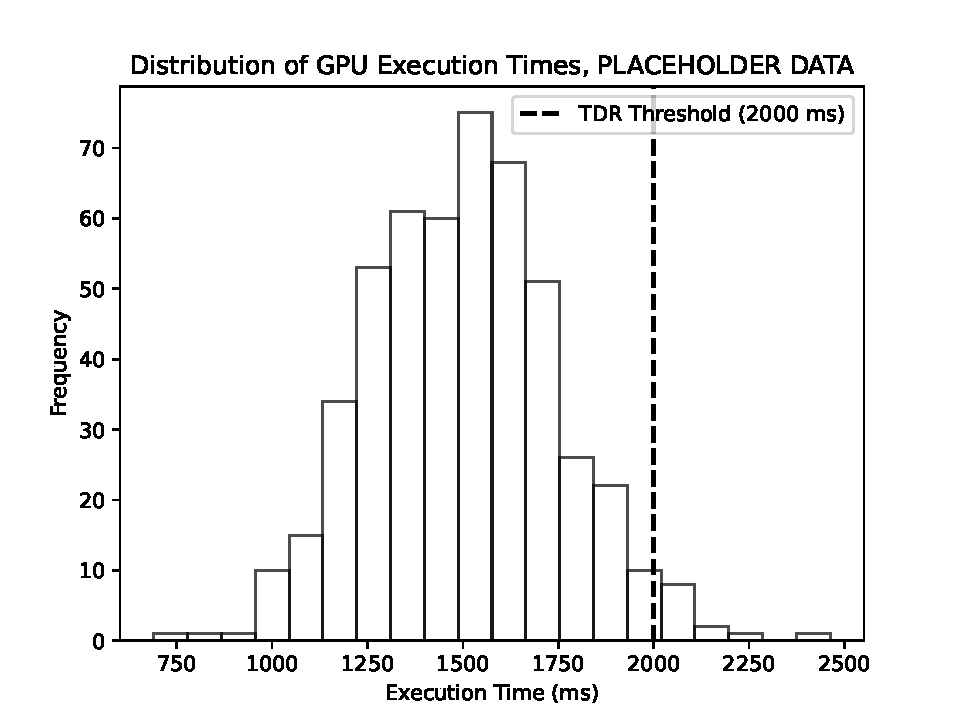
\includegraphics[width=\linewidth]{graphics/Figure_1.pdf}
  \caption{Execution times of \emph{Decoupled-Lookback (PLACEHOLDER DATA)}}
\end{figure}

Exacerbating this issue is the fact that no major graphics API currently provides developers with a mechanism to query FPG support. This lack of transparency forces developers to design algorithms without clear knowledge of whether critical guarantees are available on the target hardware. In environments like shading languages, where cross-platform portability is required, this uncertainty compels developers to revert to older, less efficient strategies such as \emph{Reduce-Then-Scan}. Yet, in the absence of guaranteed forward progress, developers have little choice but to sacrifice performance for broader compatibility.

\subsection{Earlier Attempts at Portability}
Levien and Naur~\cite{Raph2021} made the first attempt at implementing a \emph{DecoupledLookback} approach without forward progress requirements in \emph{ScalarFallback}. By allowing a workgroup to access and operate on another tile’s data, \emph{ScalarFallback} targets the mutual exclusion condition outlined by Coffman et al., ensuring that no single workgroup holds exclusive control over a resource. Instead, each time a workgroup spins on a preceding tile, it advances a \emph{fallback} operation by incrementally consuming the blocking tile---one element at a time. Although this entails performing redundant work when the blocking tile is simply late but not deadlocking, it guarantees the termination of the algorithm because a workgroup can perform the reduction of a blocking tile itself, breaking the inter-workgroup dependency.

\emph{ScalarFallback} suffers from two primary issues that impact its efficiency. First, the fallback reduction is performed serially by a single thread, progressing only when the workgroup engages in a waiting spin. This effectively takes $t$ spins to complete the fallback of a deadlocking $t$-sized tile. Moreover, because only a single thread is responsible for loading elements, the cache line associated with the loaded elements is severely underutilized, further degrading performance. Second, once the fallback is complete, the workgroup does not post its result to device memory. Consequently, every workgroup deadlocked by that tile must redundantly execute the fallback, wasting computational resources. While \emph{ScalarFallback} was able to achieve speed of light on hardware supporting FPG and executed correctly on hardware without FPG, its performance on the latter was inferior to that of \emph{Reduce-Then-Scan}.

\section{Design}
\thomas{I've broken somewhat with the outline and moved the goals and non-goals section to somewhere in the introduction. I kept finding myself trying to write around it. I think the content there is good, but it's very awkward as it ended up so deep within the paper. The placement of this section here feels more natural, and seems to mirror other papers?}

\subsection{Breaking Deadlocks}
\thomas{What I want to accomplish here is to go beyond saying "Here is our method. It works great." I want to show that these are the possible avenues to attack deadlocking . . . and exhaustively demonstrate that removing  Coffman's mutual exclusion is the best way to do it, under our given constraints.}

Deadlock in \emph{Chained-Scan} arises from the inter-workgroup dependencies that are inherent to scan operations. These dependencies are governed by Coffman et al.'s~\cite{10.1145/356586.356588} four necessary conditions for deadlock: \emph{mutual exclusion}, \emph{resource holding}, \emph{no preemption}, and \emph{circular dependency}. While all four conditions are theoretically avenues for addressing deadlock, practical constraints and the requirements of \emph{Chained-Scan} significantly narrow the set of viable approaches.

The first condition, \emph{dependency relationships}, is immutable in the context of scan operations. Similarly, \emph{no preemption} is immutable within the GPU programming model. Addressing \emph{resource holding} by allowing workgroups to release resources (losing context) during waits effectively reintroduces kernel launches as inter-workgroup barriers. Designing tile sizes to break \emph{circular dependency} by mapping workgroups one-to-one with multiprocessors might seem feasible but is impractical. GPU vendors provide no guarantees regarding workgroup progress behavior, leaving starvation risks unresolved. Moreover, such strategies are non-portable and contradict the goal of supporting diverse hardware architectures.

\subsection{Decoupled-Fallback}

\section{Implementation}
We are in WGSL. We don't have: a memory model, 64-bit atomics, and atomicCAS is unreliable. 

\subsection{Split Method}
\begin{enumerate}
    \item Idea: Split the reductions into multiple values; use separate values for local/inclusive instead of using flags to differentiate them.
    \item Pro: Full 32 or theoretically 64 bits.
    \item Pro: No memory model or 64 bit atomics required!
    \item Pro: Can safely fallback insert without risking clobbering.
    \item Con: 2x Memory usage
    \item Con: Places subgroup functions adjacent to atomics, which may lead to \textbf{\textit{interesting}} behavior.
\end{enumerate}

\begin{figure}[h]
  \centering
  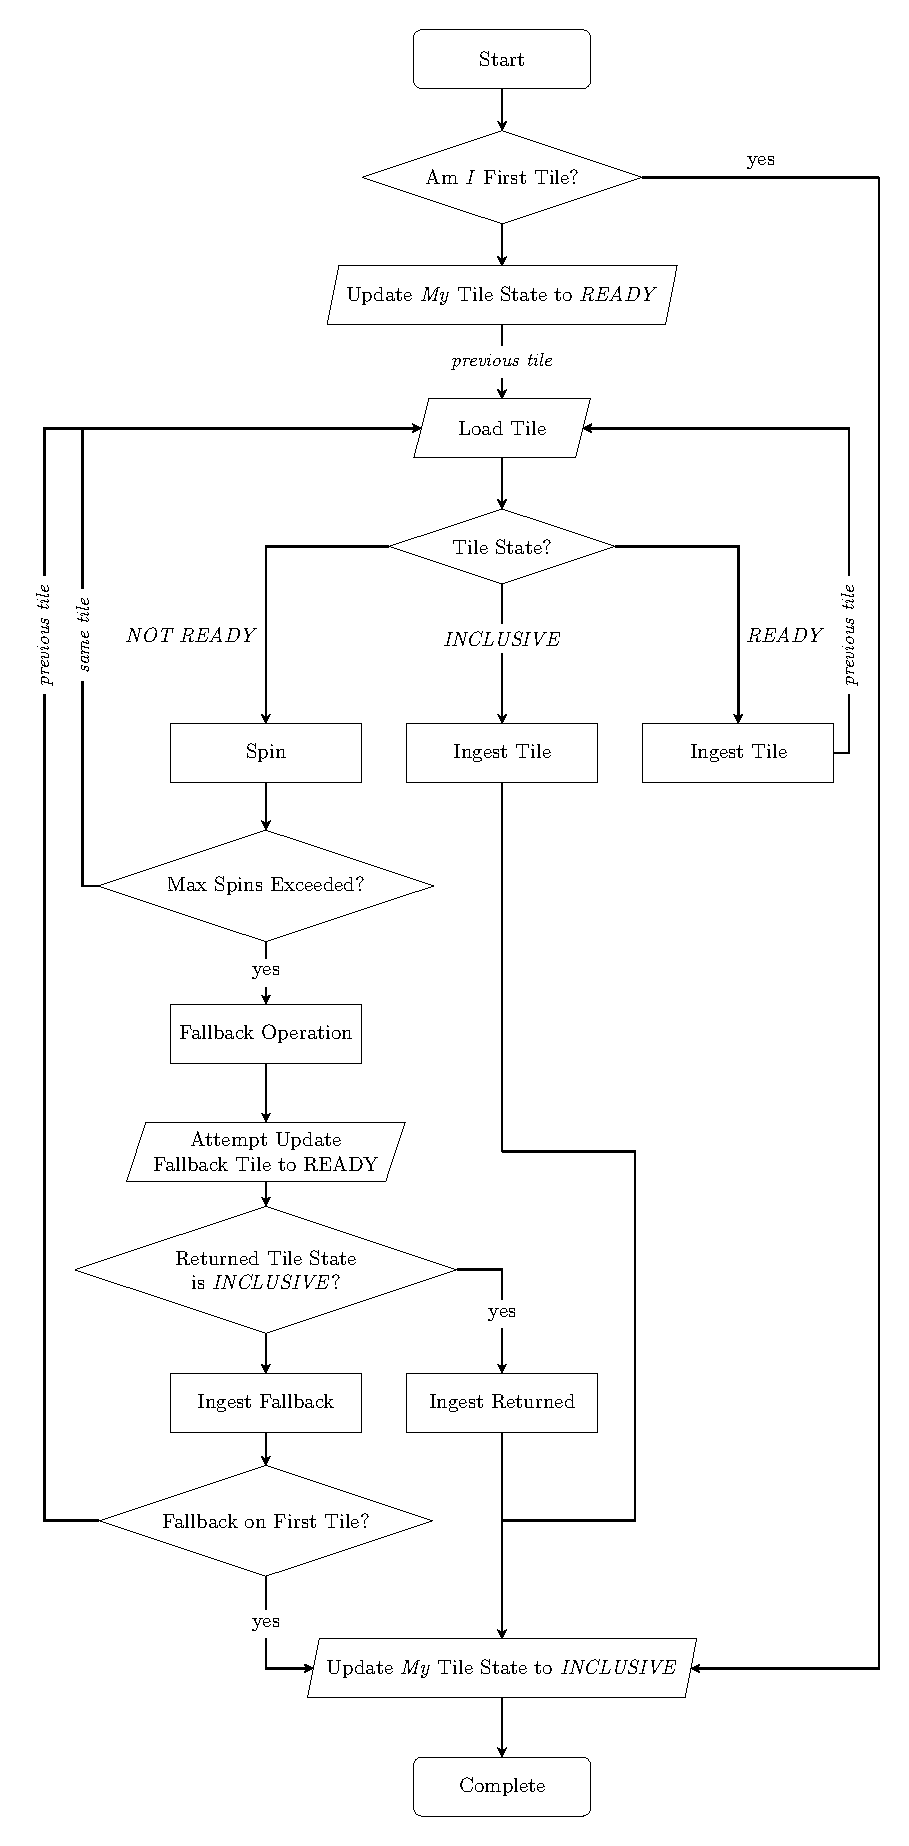
\includegraphics[width=\linewidth]{graphics/FlowChart.pdf}
  \caption{TODO update for split}
\end{figure}

\subsection{Intra-Workgroup Scan}
Our intra-workgroup implementation is most similar to the \emph{CUDPP}~\cite{} scan kernel, with adaptations to enhance portability. It consists of three phases:
\begin{enumerate}
  \item
\end{enumerate}

The WebGPU specification supports subgroup sizes $s$, where $s = 2^k$ and $k \in [2, 7]$; on some hardware, subgroup sizes can vary between kernel launches. To handle this variability, we use a generalized radix-$s$ Ladner-Fischer scan network embedded with Kogge-Stone subgroup scans to perform the scan on the intra-workgroup spine. The upsweep phase of the Ladner-Fischer network follows a Brent-Kung~\cite{1675982} construction; assuming shared memory bank widths equal to the subgroup size, any subgroup scans beyond the first will experience maximum $s$-way bank conflicts. To mitigate this, we employ a Merrill-Grimshaw~\cite[Section 3.3.5]{Merrill2009} style conflict avoidance strategy, which reduces bank conflicts to the radix base of the network—in our case, $s$. Counterintuitively, the resulting $s$-way conflict differs from the conflicts incurred by the Brent-Kung construction. Rather than multiple threads accessing different indices in the same memory bank, this conflict arises from a fanout originating from a single index. However, such access is interpreted by the hardware as a broadcast operation, resulting in no conflicts. Thus, this network offers several advantages: minimal depth of $\log_2 n$; asymptotically optimal $O(n)$ size; zero bank conflicts across all supported subgroup sizes.

\begin{algorithm}[htbp]
  \SetAlgoLined
  \KwIn{Shared Memory Array to Scan $x$, Workgroup Size $W$, Subgroup Size $S$}
  \KwOut{Shared Memory Inclusive Scanned Array $x$}

  $spine\_length \gets W / S$\;
  $alignment \gets 1 << \text{divRoundUp}(\log_2(spine\_length), \log_2(S)) * \log_2(S)$\;

  $stride \gets 1$\;
  $top\_offset \gets 0$\;

  \ForEach{$thread\_id$ \textbf{in} $W$ \textbf{in parallel}}{
    \For{$j \gets S$ \KwTo $alignment$ \textbf{with} $j \gets j * S$}{

      $step \gets spine\_length / stride$

      \If{$thread\_id < step$}{
        $temp \gets \text{subgroupInclusiveScan}(x[thread\_id + top\_offset])$\;
        $x[thread\_id + top\_offset] \gets temp$\;
        \If{$\text{\normalfont highestRankLane}(thread\_id)$}{
          $x[(thread\_id / S) + step + top\_offset] \gets temp$;
        }
      }

      \textbf{barrier()}\;

      \If{$j \neq S$}{
        $reduced\_stride \gets j / stride$\;
        $fanout\_index \gets thread\_id + reduced\_stride$\;

        $cond1 \gets fanout\_index < spine\_length$\;
        $cond2 \gets (fanout\_index \& (j - 1)) \geq reduced\_stride$\;

        \If{$cond1 \textbf{ \&\& } cond2$}{
          $x[fanout\_index] \gets x[fanout\_index] + x[((fanout\_index / stride) + top\_offset) - 1]$\;
        }
      }
      $stride \gets stride * S$\;
      $top\_offset \gets top\_offset + step$\;
    }
    \textbf{barrier()}\;
  }
  \Return{$x$}\;
  \caption{Subgroup-Size-Agnostic Scan}
  \label{alg:example}
\end{algorithm}

\subsection{Work Efficiency and Depth}
\subsubsection{Subgroup Raking}

\subsubsection{Size Agnostic Scan}
For a subgroup of size $s$, the Kogge-Stone network has a work complexity of $s \log_2 s$. Given an input of size $n$, the work complexity is:
\begin{equation}
  \begin{aligned}[b]
    \text{Work} & = \underbrace{\vphantom{\sum_{k=0}^{\lceil \log_s n \rceil}}n}_{\text{fanout}}
    +
    \underbrace{\sum_{k=1}^{\lceil \log_s n \rceil}}_{\text{iterations}}
    \underbrace{\vphantom{\sum_{k=1}^{\lceil \log_s n \rceil}}\frac{n}{s^k}}_{\text{calls per iteration}}
    \cdot
    \underbrace{\vphantom{\sum_{k=1}^{\lceil \log_s n \rceil}}s \log_2 s}_{\text{work per call}} \\
                & = n + s \log_2 s \cdot \sum_{k=1}^{\lceil \log_s n \rceil} \frac{n}{s^k}       \\
                & = O\left(n + n \log_2 s\right)                                                 \\
                & = O(n \log_2 s).
  \end{aligned}
\end{equation}
Since the subgroup size remains constant within each kernel launch, the final work complexity is $O(n)$. Thus our implementation preserves asymptotically optimal work, even though the structure is not isomorphic to the radix-two network. The Kogge-Stone scan has a depth of $\log_2 s$ Thus, the total depth of the scan is:
\begin{equation}
  \begin{aligned}[b]
    \text{Depth} & = \underbrace{\lceil \log_s n \rceil}_{\text{loop iterations}}
    \cdot \underbrace{\log_2 s}_{\text{depth per iteration}}                           \\
                 & = \left\lceil \frac{\log_2 n}{\log_2 s} \right\rceil \cdot \log_2 s \\
                 & = \log_2 n + O(1).
  \end{aligned}
\end{equation}
While minimal depth is preserved regardless of the subgroup size, this result can be somewhat misleading, as the depth incurred during the subgroup portion of the scan requires no barrier, whereas the main loop incurs a workgroup-wide barrier at each iteration. Consequently, while the theoretical depth remains constant across subgroup sizes, smaller subgroups tend to perform worse in practice due to the increased relative cost of synchronization and the overhead of additional iterations in the main loop.

\subsubsection{Full Algorithm}

\section{Experimental Setup}

\section{Results and Analysis}

\section{Discussion}

\subsection{Trade-offs}

\subsection{Limits on Speed-of-Light Performance}
There are a number of factors which may preclude speed-of-light performance, but most salient is the fairness of the scheduling model. In \emph{Decoupled-Fallback}, a work tile which is late due to unfairness is indistinguishable from one which is deadlocking, so as a scheduler becomes increasingly unfair, it incurs an increasing number of redundant fallbacks. Consider a hardware with a workgroup occupancy denoted by $o$, and let $f$ represent the probability that a fallback operation occurs at a particular lookback step. Because the number of lookback steps is bounded by $o$, the expected number of fallback operations is approximately $fo$. This results in a factor of $fo$ increase in global memory reads and a factor of $fo\log{n}$ increase in work.

This increased sensitivity to fairness exacerbates existing issues which negatively impact the performance of previous scan architectures, namely lack of compute, and slow atomic update latency. On hardware that lacks sufficient compute power to be memory-bandwidth bound, the additional work incurred by redundant fallback reductions is particularly deleterious. High atomic update latency further compounds the problem: as inter-workgroup communication time grows, the minimum delay before updates become visible to dependent workgroups also increases. This, in turn, raises the number of lookback steps that may be needed and potentially leads to redundant fallbacks.

\section{Cut material, can be readded if we have enough space}

To ensure consistency with our coding artifact and promote cross-vendor compatibility, we use the terminology of the WebGPU specification.
\setlength{\tabcolsep}{3pt}
\begin{table}[h]
  \centering
  \caption{Non-Exhaustive Equivalent Terminology}
  \label{tab:terminology}
  \begin{tabular}{lcccc}
    \toprule
    \textbf{WGSL}   & \textbf{GLSL}  & \textbf{HLSL}   & \textbf{Metal}     & \textbf{CUDA} \\ \midrule
    Subgroup        & Subgroup       & Wave            & SIMD-group         & Warp          \\
    Workgroup       & Workgroup      & Group           & Threadgroup        & Block         \\
    Workgroup       & Shared         & Groupshared     & Threadgroup        & Shared        \\ \bottomrule
  \end{tabular}
\end{table}

Despite its limited suitability within the oversubscription paradigm, inter-workgroup synchronization holds significant performance potential, as many GPU-friendly algorithms—such as \emph{example}, \emph{example}, and \emph{scan}---can benefit from a trade-off that eliminates the costly overhead of kernel-launch synchronization. This potential was explored in prior work~\cite{}, culminating in Gupta et al.’s~\cite{} \emph{Persistent Thread} paradigm. Rather than oversubscribing processors by launching $b$ workgroups, each consuming a single \emph{work tile}, this approach \emph{discovers} the total workgroup occupancy across the device $o$---referred to by Gupta et al. as a \emph{maximal launch}---and launches $o$ workgroups, each responsible for processing $b/o$ work tiles. Limiting the launch size allows the workgroups to always remain on chip, eliding context switching, and thus facilitating an efficient inter-workgroup barrier.

\begin{acks}
\end{acks}

\bibliographystyle{ACM-Reference-Format}
\bibliography{bib}

\appendix

\section{Research Methods}

\end{document}
\endinput

%%% Local Variables:
%%% mode: LaTeX
%%% TeX-master: t
%%% End:
